\chapter{Probabilistic Models}

\section{Modeling with Probability Distributions}

% a discussion on binomial distribution.
The normal rate of infection of a certain disease in cattle is
25\%.  Each animal becomes infected (or not) independently of other
animals.  A team of veterinarians would like to test a new
vaccine. Which of the following two scenarios, \ref{sc1} or \ref{sc2},
provides more evidence that the vaccine is effective.  \emph{Hint:}
Compute the probability that each scenario would occur under the
hypothesis that the vaccine has no effect whatsoever.
\begin{enumerate}[A)]
\item 10 animals are vaccinated and none of them become infected. \label{sc1}
\item 17 animals are vaccinated. At most one of the animals becomes infected. \label{sc2}
\end{enumerate}

Let $X$ be the number of animals infected under the assumption that
the vaccine is worthless.  Under scenario \ref{sc1},
\[ X \sim \text{Binomial}(n=10,p=.25) \]
\[ P(X = 0) = {10 \choose 0} .25^0 .75^{10} = .0563 \]
Under scenario \ref{sc2}, 
\[ X \sim \text{Binomial}(n=17,p=.25) \]
\begin{align*} P(X \leq 1) &= P(X=0) + P(X=1) \\
                 &= \sum_{x=0}^1 {17 \choose x} .25^x .75^{17-x} \\
                 &= .0501
\end{align*}
In the absence of a working vaccine, scenario \ref{sc2} is less likely to occur,
and so it provides a better test of the effectiveness of the vaccine.


% use this section to illustrate modeling with a poisson rv
At a facility that manufactures recreational sports
  vehicles (ATVs), each vehicle is subjected to a final
  inspection. The rate of defects during final inspection is
  $\lambda=1.5$ defects per vehicle.
\begin{enumerate}
\item What is an appropriate probability distribution to model the
number of defects? \label{atv1}
\item What proportion of vehicles have more than 2 defects? \label{atv2}
\item Management has set a new goal that the proportion
of vehicles with no defects is .5. What rate $\lambda$ would
achieve this goal? \label{atv3}
\end{enumerate}

We are interested in the number of defects, which is discrete.
The Poisson distribution makes sense because it is commonly used
for count data. Moreover, we are given information for a single
parameter, and the Poisson distribution has a single parameter.
If we let the random variable $X$ represent the number of defects
per vehicle, then a reasonable distribution is
\[ X \sim \text{Poisson}(\lambda=1.5) \]
For part~\ref{atv2},
\begin{align*}
P(X>2) &= 1 - P(X \leq 2)\\
       &= 1 - \sum_{x=0}^2 \frac{e^{-\lambda}\lambda^x}{x!}\\
       &= 0.191
\end{align*}
For part \ref{atv3}, management's goal is that $P(X=0)=0.5$, or
\[ P(X=0) = \frac{e^{-\lambda}\lambda^0}{0!} = e^{-\lambda}=0.5 \]
Then
\[ \lambda = -\ln{0.5} = 0.693 \]

%% using poisson distribution and binomial distribution, and independence
The number of bacteria colonies of a certain type in samples of
polluted water has a Poisson distribution with a mean of 2 per cubic
centimeter. If four 1--cubic--centimeter samples are independently
selected from this water, find the probability that at least one
sample will contain one or more bacteria colonies.

Let $X$ be a random variable that represents the number of bacteria
colonies in a 1 cm$^3$ sample of the polluted water. From the problem
description,
\[ X \sim \text{Poisson}(\lambda = 2) \]
First let's find the probability that any particular sample will contain
at least one colony.
\begin{align*}
  P(X \geq 1) &= 1 - P(X=0)\\
              &= 1 - \frac{e^{-\lambda}\lambda^0}{0!}\\
              &= 1 - e^{-2}\\
  &= .865
\end{align*}
Now, the four samples are independent and the the probability that
a sample contains one or more colonies is the same for each sample.
Let $Y$ be a random variable that represents the number of samples
that contain one or more colonies. Then
\[ Y ~ \sim \text{Binomial}(n=4, p=0.865) \]
and we want to know $P(Y \geq 1)$.
\begin{align*}
  P(Y \geq 1) &= 1 - P(Y = 0)\\
              &= 1 - {4 \choose 0} (.865)^0 (1 - .865)^4 \\
  &= 0.9997
\end{align*}

% discussion on the Normal distribution
A refinery makes two grades of gasoline, regular and premium.  The
advertised octane ratings are 87 for regular gasoline and 89 for
premium gasoline.  The quality engineer at the refinery asks for 10
samples from one of the two types of gasoline. She does not know for
sure whether the samples are from the regular batch or the premium
batch. She devises the hypothesis test
\begin{align*}
H_0: \mu &\leq 87 \\
H_1: \mu &> 87
\end{align*}
and sets the confidence level to be 0.995. Suppose that the mean of
the 10 samples is 88.3 and the standard deviation is 1.0. What is her
conclusion for the hypothesis test?

Suppose that a gas station owner has his own octane test
kit and rule for accepting a tanker-truck of premium gasoline.
The owner knows from past shipments that the distributions
of octane ratings are
\begin{align*}
X_{\text{regular}} &\sim N(87,1) \\
X_{\text{premium}} &\sim N(89,1)
\end{align*}
Although the owner may not think about it explicitly, his hypothesis
test is
\begin{align*}
H_0: \mu &= 87 \\
H_1: \mu &= 89
\end{align*}
The owner takes one sample from the tanker-truck. If the octane
measurement is greater than 88.5, then he will accept the shipment as
premium gasoline. What is the probability that the owner accepts a
shipment of regular gasoline as premium (i.e. what is $\alpha$)? What
is the probability that he declines a shipment of premium gasoline,
claiming that he thinks it is regular (i.e. what is $\beta$)?  Use the
Normal distribution for this problem. The following diagram may help.

\begin{tikzpicture}
\begin{axis}[
  no markers, domain=0:12, samples=100,
  height=5cm, width=15cm,
  axis x line=bottom,
  axis y line=none,
  xtick=\empty, ytick=\empty,
  extra x ticks={4,6,7},
  extra x tick labels={87,88.5,89},
  enlargelimits=false, clip=false
  ]
  
  \addplot [fill, pattern=north west lines, domain=0:6] {gauss(7,1)} \closedcycle;
  \addplot [fill, draw=none, domain=6:12] {gauss(4,1)} \closedcycle;
  \addplot [thick] {gauss(4,1)};
  \addplot [thick] {gauss(7,1)};

  \draw [ultra thin] (4,0) -- (4,.3989);
  \draw [ultra thin] (7,0) -- (7,.3989);

  \draw (4,.42) node[anchor=south] {$H_0$};
  \draw (7,.42) node[anchor=south] {$H_1$};

  \draw (4.9,.15) node[anchor=east] (beta) {$\beta$};
  \draw (5.4,.03) node (beta2) {};
  \draw[-] (beta) -- (beta2);

  \draw (6.5,.15) node[anchor=west] (alpha) {$\alpha$};
  \draw (6.1,.005) node (alpha2) {};
  \draw[-] (alpha) -- (alpha2);
  
\end{axis}
\end{tikzpicture}

For the quality engineer, the test statistic is
\[
t_0 = \left( \overline{X} - \mu_0 \right)\frac{\sqrt{n}}{S} 
= \left(88.3 - 87\right) \frac{\sqrt{10}}{1} 
 = 4.11
\]
and since $t_0 > t_{\alpha,n-1}=3.25$ ($\alpha=0.005$) she will
reject $H_0$ and conclude that the samples are from the premium
batch of gasoline.

For the station owner,
\begin{align*}
\alpha &= P(X > 88.5 \mid H_0) \\
&= P\left( Z > \frac{88.5-87}{1} \right) \\
&= 1 - P(Z < 1.5) \\
&= 0.067
\end{align*}
and
\begin{align*}
\beta &= P(X < 88.5 \mid H_1) \\
&= P\left( Z < \frac{88.5-89}{1} \right) \\
&= P(Z < -0.5) \\
&= 0.309
\end{align*}

\section{Stochastic Processes}

% Use this section to introduce the idea of a Poisson Process.
% add explanatory material.
\emph{A Poisson Process.} A statistician has observed the behavior of
a Hollywood celebrity for about one year and has noted that between
the hours of 8pm and 11pm this celebrity generates, on average, three
tweets per hour and that the rate is approximately the same within
each one-hour period.  We can count the \emph{number} of tweets that
occur in a time interval $t$. We can also measure the \emph{time}
between tweets. Here is a depiction of the tweets from last night.

\vspace{.2in}
\begin{center}
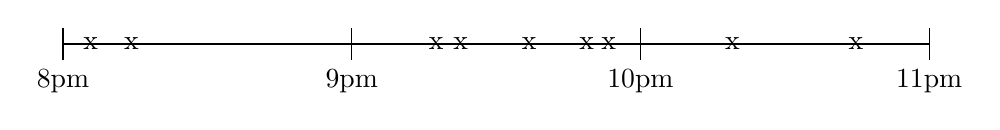
\begin{tikzpicture}

\draw (0,0) -- (11,0)
  node[pos=0.35/11]{x}
  node[pos=0.87/11]{x}
  node[pos=4.74/11]{x}
  node[pos=5.05/11]{x}
  node[pos=5.92/11]{x}
  node[pos=6.65/11]{x}
  node[pos=6.93/11]{x}
  node[pos=8.50/11]{x}
  node[pos=10.07/11]{x}
;
\node[below] at (0,-.2) {8pm};
\draw (0,-.2) -- (0,.2);
\node[below] at (11/3,-.2) {9pm};
\draw (11/3,-.2) -- (11/3,.2);
\node[below] at (22/3,-.2) {10pm};
\draw (22/3,-.2) -- (22/3,.2);
\node[below] at (11,-.2) {11pm};
\draw (11,-.2) -- (11,.2);


\end{tikzpicture}
\end{center}

Let the random variable $Y$ be the number of tweets from
the celebrity in some time interval.
When we say that the number of tweets in a time interval $t$ follows
a Poisson distribution with mean $\lambda t$, we write
\[
  Y \sim \text{Poisson($\lambda t$)}
\]
If $t$ is one hour, then we can write
\[
  Y \sim \text{Poisson($\lambda = 3$)}
\]
Stating that the number of tweets follows a Poisson distribution
implies that the time between tweets follows an Exponential
distribution (and vice versa). Let the random variable $X$ be
the time between tweets. Then
\[
  Y \sim \text{Poisson($\lambda t$)} \Longleftrightarrow X \sim \text{Exp($\lambda$)}
\]
Yes, it is the same $\lambda$ in each distribution.
The average number of tweets is $\lambda=3$ per hour. The average
time between tweets is $1/\lambda = 1/3$ hour (or 20 minutes).
Recall that for the Exponential distribution
\[
  E(X) = \frac{1}{\lambda} = \frac{1~\text{hour}}{3~\text{tweets}} = 20 ~\text{minutes per tweet on average}
\]

Questions.
\begin{enumerate}
\item What is the probability that the celebrity sends out five or
  more tweets in one hour?
\item What is the probability that the celebrity sends out
  no tweets between 9pm and 11pm?
\end{enumerate}

\section{Queueing Models}

\section{Stochastic Dynamic Programming}

\section{Probabilistic Inventory Models}

% first we need to introduce the newsvendor problem.
% perhaps solve this problem as a newsvendor problem.
% also need to make sure that the example of turkeys is OK to use.

\emph{Monte Carlo simulation and Thanksgiving turkeys.}
Tom the grocer pays \$10 wholesale for his turkeys.  Before
Thanksgiving he sells them for \$18.  After Thanksgiving he sells any
remaining turkeys for \$5 each.  In the past years Tom has noticed
pre-Thanksgiving demand has varied uniformly between 50 and 100 birds.
How many turkeys should he buy to maximize his expected profit?

Let's let $x$ represent the number of turkeys that Tom should order.
The random pre-Thanksgiving customer demand is $D$, and Tom's
expect profit is $P$, where

\begin{equation*}
  P = \begin{cases}
    (18 - 10)x & \text{if}~D \geq x \\
    18D - 10x + 5(x - D) & \text{if}~D < x
  \end{cases} 
\end{equation*}
           
Let's find an optimal value for $x$ (our decision variable)
via simulation. Here are the steps.

\begin{compactenum}
\item Set $x = 50,~51,~52,~\ldots,~100$.
  \begin{compactenum}
\item For each value of $x$ generate $B \approx 200$ independent replications
  of $D$, where $D \sim U(50,~100)$. Call the realized values of demand $D_i$ where
  $i = 1 \ldots B$.
\item Calculate the profit $P_i$ for each $D_i$.
  \end{compactenum}
\item Estimate expected profit for each value of $x$ as
  \[ \frac{1}{B} = \sum_{i=1}^B P_i \]
\item Choose the value of $x$ that achieves the maximum profit.
\end{compactenum}

An implementation in R is shown in Figure~\ref{fig:sim-turkeys} and the
output is shown in Figure~\ref{fig:plot-turkeys}.

\begin{SaveVerbatim}{simulation}
Order <- 50:100
EP <- numeric(length(Order))  # will hold expected profit
B <- 200                      # number of replications

for (x in Order) {
    P <- numeric(B)   # will hold realized profits
    for (i in 1:B) {
        D <- sample(50:100, 1)
        if (D >= x) { # sell all turkeys
            P[i] <- 8*x
        } else {      # don't sell them all
            P[i] <- 18*D - 10*x + 5*(x-D)
        }
    }
    EP[which(x==Order)] <- mean(P)
}

plot(Order, EP)   # using base R graphics
\end{SaveVerbatim}

\begin{figure}
\fbox{
\begin{minipage}{\textwidth}
\BUseVerbatim{simulation}
\caption{Simulation to determine the number of turkeys to order
  so that expected profit is maximized.}
\label{fig:sim-turkeys}
\end{minipage}
}
\end{figure}

\begin{figure}
\begin{center}
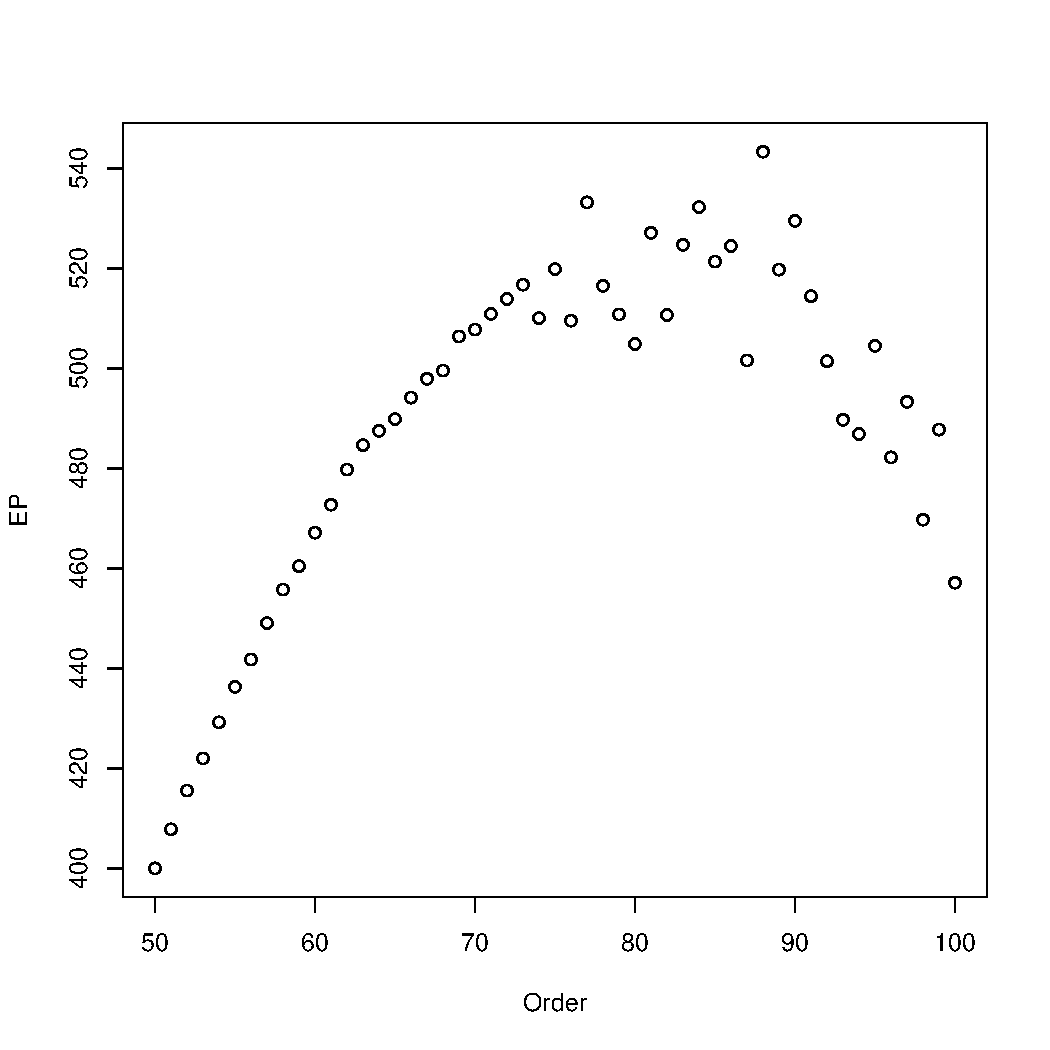
\includegraphics[width=0.7\columnwidth]{turkeyprofit.pdf}  % change to tikz plot with data
\caption{Plot of expected profit vs. turkeys ordered.}
\label{fig:plot-turkeys}
\end{center}
\end{figure}

\emph{Questions.}
\begin{enumerate}
\item Referring to Figure~\ref{fig:plot-turkeys}, why does it appear
  that the expected profit is becoming more varied as the order
  quantity increases? What can we do about it?
\item Can you solve this problem analytically?
\item Why use simulation?
\end{enumerate}

\emph{Auctioning a turkey.}
On the Wednesday before Thanksgiving, Tom decides to auction a turkey
with the proceeds donated to charity. Tom will offer the turkey using
a second-price sealed-bid auction. In a second-price auction
(also valled a Vickrey auction), the highest bidder wins, but the pays the
price of the second-highest bid.  At the time of the auction it turns
out that there are only two bidders.  Tom doesn't want to give the
turkey away so he sets a reserve price $r$.  The reserve price 
modifies the rules of the auction as follows.  If both bids are below
$r$ then neither bidder wins, and Tom collects no proceeds.
If both bids are at or above $r$ then the regular 2nd-price
auction rules prevail. If only one bid is at or above $r$ then that
bidder wins the turkey and pays $r$. Both bidders agree to the rules.

Now, it is well-known that a 2nd-price is a truth-telling mechanism.
That is to say, bidders will bid their true valuations for the item.
Suppose each bidder has a value for the Turkey is independently and
uniformly distributed between \$0 and \$20.
What is the optimal reserve price $r$?

With some effort, this problem can be solved analytically.
Alternatively, and with not as much effort, we can determine the
optimal reserve price via simulation (see Figure~\ref{fig:auction}.)
Now consider adding just a bit more complexity to the problem, e.g. a
third-price auction, or multiple classes of bidders having different
valuation distributions (Gamma, Lognormal, etc.) The problem can
become intractable to solve analytically, but it is relatively easy to
obtain an approximate optimal solution via simulation.

\begin{SaveVerbatim}{auction}
auction <- function(r) {
    b1 <- runif(1, 0, 20) # bidder 1's valuation
    b2 <- runif(1, 0, 20) # bidder 2's valuation, independent of bidder 1
    if (b1 < r && b2 < r) {
        rev <- 0
    } else if (b1 >= r && b2 >= r) {
        rev <- min(b1,b2) # regular 2nd price auction
    } else {
        rev <- r
    }
    rev
}

reserve <- seq(0, 20, by=.1)
expected.rev <- numeric(length(reserve))

for (i in 1:length(reserve)) {
    expected.rev[i] <- mean(replicate(10000, auction(reserve[i])))
}

plot(reserve, expected.rev, type="l")
\end{SaveVerbatim}

\begin{figure}[h]
\fbox{
\begin{minipage}{\textwidth}
\BUseVerbatim{auction}
\caption{Implementation of a 2nd-price auction with a reserve price $r$ and
  independent valuations for two bidders. We would like to know the reserve
  price $r$ that maximizes revenue for the seller.}
\label{fig:auction}
\end{minipage}
}
\end{figure}


\section{Exercises}

\begin{enumerate}
  
\subsubsection*{Modeling with Probability Distributions.}

% this problem is OK
% geometric distribution
\item \emph{Searching for an item.} Albert has \num{1176} Pok\'{e}mon
  cards in total.  Pok\'{e}mon EX is a special type of card, and
  Albert has 39 EX-type cards.  He is looking for an EX-type card, but
  all of the cards are completely mixed up and stored in a shoe
  box. His mother is calling him for dinner.  What is the probability
  that Albert will have to look through no more than 25 cards before
  he finds an EX-type card?

\begin{solution}
\bs Consider finding an EX-type card to be a ``success''. Let $X$ be a
random variable that represents the number of cards that Albert has to
handle up to and including the first success. Then
\[
X \sim \text{Geometric}(p=\frac{39}{1176})
\]
and
\[
P(X \leq 25) = 1 - (1 - p)^{25} \approx 0.57.
\]
\end{solution}

% this problem is OK
% Binomial, odds, probabilities
\item \emph{Playing Pok\`{e}mon.} Albert is playing
  Pok\'{e}mon cards with his friend. It's Albert's turn, and he
  decides to use Marowak. The card says the following.
\begin{quote}
\emph{Flip a coin four times. The amount of damage done to your opponent's
Pok\'{e}mon is the number of heads times 40.}
\end{quote}
What are the odds that Marowak will do at least 120 damage to the
opponent? One approach to answer this question is to use the Binomial
distribution to compute the probability of doing at least 120 damage
and then convert from probability to odds. You can take another
approach if you prefer. In any case, assume that the coin is fair,
i.e.\ the probability of getting heads on any particular toss is 1/2.

\begin{solution}
\bs
In order to do at least 120 damage, we need either three or four heads
out of the four coin tosses. Let $X$ represent the number of heads obtained
in four tosses of a fair coin. Then $X \sim \text{Binomial}(p=1/2,n=4)$.
\begin{align*}
P(X=3) + P(X=4) &= {4 \choose 3} p^3 (1-p)^1 + {4 \choose 4} p^4 (1-p)^0 \\
&= \frac{1}{4} + \frac{1}{16} \\
&= \frac{5}{16}
\end{align*}
The odds are
\[
\frac{p}{1-p} = \frac{\frac{5}{16}}{1-\frac{5}{16}} = \frac{5}{11}
\]
or 5 to 11.
\end{solution}

% binomial distribution
\item \emph{System reliability.}  A data warehouse has $n$ servers.
Each server will fail, independently, with probability $p$.
\begin{enumerate}
\item Suppose that a single functioning server can support the
  integrity of the data. What is the probability that data will be
  lost? \label{ex:p1}
\item Suppose that two functioning servers are required for data
  integrity.  What is the probability that data will be lost?
\label{ex:p2}
\end{enumerate}

\begin{solution}
  \bs For part~\ref{ex:p1}, all $n$ servers must fail for data to be
  lost.  Because failures are independent, the probability of data
  loss due to server failure is $p^n$.

For part~\ref{ex:p2}, let $X$ be the number of failed servers. $X$
has a Binomial distribution with parameters $n$ and $p$. The probability
of data loss due to server failure is
\begin{align*}
      P(X \geq n-1) &= \sum_{i=n-1}^n {n \choose i} p^i (1-p)^{n-i} \\
      &= {n \choose n-1} p^{n-1} (1-p)^{n-(n-1)} + {n \choose n} p^n (1-p)^{n-n} \\
      &= np^{n-1}(1-p) + p^n \\
      &= np^{n-1} - np^{n-1}p + p^n\\
      &= np^{n-1} - np^n + p^n\\
      &= np^{n-1} + (1-n)p^n
\end{align*}
\end{solution}

% this problem is OK
% exponential distribution
\item \emph{Evaluating a warranty.}
  A manufacturer of automotive batteries offers a one-year
  warranty. If the battery fails for any reason during the warranty
  period, it is replaced for free. The time to failure is distributed
  Exponential with rate $\lambda=.125$ failures per year.
\begin{enumerate}
\item What proportion of batteries fail within the warranty period?
\item The cost to manufacture a battery is \$50, and the profit
per battery is \$25. What is the effect of the warranty replacement
policy on profit? \label{ex:profit}
\end{enumerate}

\begin{solution}
  \bs The question is asking for the theoretical proportion of
  batteries that fail within one year. Since all batteries have the
  same probability of failure, this proportion is equal to the
  probability that a single battery will fail within one year. Let $X$
  be a random variable that represents the time to failure.
\[ P(X<1) = 1-e^{-\lambda t} = 1 - e^{-.125} = 0.118 \]
Now, imagine that the manufacturer has, over time,
  sold many batteries and has kept data on how many batteries failed
  within one year. The empirical proportion is simply the number
  of batteries that failed divided by the number of batteries sold.
  The Law of Large Numbers tells us that when the number of batteries
  sold is large, the empirical proportion will be approximately
  equal to the theoretical proportion.

Taking the warranty into account, the average profit per battery is
\[ \$25 - 0.118\times \$50 = \$19.10 \]
So, the (average) effect of the warranty on profit is -\$5.90.
\end{solution}

% memoryless property of the Exponential distribution this problem is
% from Ross. It's a thought experiment. The actual numbers don't
% matter as long as the rates are the same. Can we find a different
% scenario that illustrates the same idea: the memoryless property
\item \emph{Memoryless property of the Exponential distribution.} A
  hair salon has two hairdressers who provide haircuts on a walk-in
  basis. Sam arrives to the salon and finds that both hairdressers are
  busy with customers. However, no other customers are waiting, so Sam
  will begin his haircut (immediately) when the first space opens up.
  Suppose that the distribution of service times for both hairdressers is
  exponential with rate $\lambda$. What is the probability that
  Sam is the last of the three customers to complete a haircut?

\begin{solution}
  \bs By the memoryless property of the Exponential distribution, the
  distribution of remaining time for each customer currently receiving
  a haircut is exponential with rate $\lambda$.  Since the two
  customers getting haircuts have the same distribution for remaining
  time, the probability that customer 1 finishes before customer 2 is
  1/2 (likewise for customer 2 finishing before customer 1). When Sam
  enters service, the memoryless property still applies.  Regardless
  of how long the other customers have been in service, Sam has the
  same distribution for remaining time. The probability Sam is the
  last to finish is 1/2.
\end{solution}

% Poisson distribution
\item \emph{Donut giveaway.}  A professional baseball team has just
  won a game that secured them a berth in the league’s playoffs. To
  celebrate, a local donut shop will be giving away up to 200 free
  donuts during a two-hour period on the morning following the
  victory. All 200 donuts will be baked and decorated with a baseball
  theme before the giveaway starts. If there are any donuts remaining
  after the giveaway, they will be sold at a discounted price. Assume
  that customers will arrive at the giveaway according to a Poisson
  process at a mean rate of 100 customers per hour. Also, note that
  there is a limit of one donut per customer.
\begin{enumerate}
\item What is the probability that there will be donuts remaining
  after the giveaway? \label{ex:donuta}
\item What is the predicted number of donuts that will be remaining
  after the giveaway? \label{ex:donutb}
\end{enumerate}

For part~\ref{ex:donuta}, present your answer as an expression for the
probability that there will be donuts remaining. Then, use software,
such as R, to compute a numerical answer.

\begin{solution}
  \bs Given that customers arrive to the giveaway according to a
  Poisson process with a mean of 100 customers per hour, the number of
  customers that arrive during the two-hour period is Poisson
  distributed with a mean of 200. Let $N$ be the number of customers
  arriving in a two-hour period. Then
  \[ N \sim \text{Poisson}(\lambda = 200) \] 
For part~\ref{ex:donuta},
  the probability that there will be donuts remaining after the
  giveaway is
\begin{align*}
P(N < 200) &= \sum_{n=0}^{199} \frac{\lambda^n e^{-\lambda}}{n!}\\
&= \sum_{n=0}^{199} \frac{200^n e^{-200}}{n!}\\
&\approx .49
\end{align*}
In R,
\begin{Verbatim}
> sum(dpois(0:199,200))
[1] 0.4905966
\end{Verbatim}  

For part~\ref{ex:donutb}, our calculations are all done in expectation
(that is to say, on average). There are 200 customers in 2 hours,
which means that 200 donuts are given away. So, on average, no donuts
remain.
\end{solution}

% re-written by hannah
% Poisson distribution
\item \emph{Startup expenses.}  Two friends are starting a small
  business selling ice cream. They applied for a grant and have
  received \$\num{1800} to help cover any startup expenses. The
  friends will incur expenses of \$300 randomly throughout the first
  year, and the time between payments for these expenses is
  exponential with a mean of 2 months. Determine the probability that
  the friends will run out of grant money before the end of the year.

\begin{solution}
  \bs Let $X$ be a random variable that represents the time between
  payments. The mean time between payments, that is to say the
  expected value of $X$ ($E(X)$), is two months. We know that for the
  Exponential distribution
  \[ E(X) = \frac{1}{\lambda} \] where $\lambda$ is the rate (in units
  of payments per month). So,
  \[ X \sim \text{Exp}(\lambda = 1/2~\text{payments per month}) \] If
  the time between payments is distributed Exponential with rate
  $\lambda$, then the number of payments in $t$ months is Poisson with
  mean $\lambda t$. Let $N$ be the number of payments in 12 months.
  \[ N \sim \text{Poisson}(\lambda t = \lambda \times 12 = 6) \] Now,
  the probability that the friends runs out of money is
\begin{align*}
      P(N \geq 6) &= 1 - P(N \leq 5) \\
      &= 1 - \sum_{n=0}^{5} \frac{\lambda^n e^{-\lambda}}{n!}\\
      &= 0.55
\end{align*}
You may have defined the event that the friends runs out of
money as $P(N = 6)$. In other words, that there are exactly
six payments during the first year.  This is incorrect because
we are modeling the spending activity as a Poisson process. In
other words, the (unstated) assumption is that the number of
payments is independent of the available funds.
\end{solution}

% re-written by hannah
% poisson distribution
\item \emph{Stocking a vending machine.}  A university cafeteria has a
  vending machine that is stocked with a variety of juices and
  sodas. A student employee replenishes inventory weekly so that there
  are 180 beverages in stock at the beginning of each week. The
  cafeteria is open 24 hours, 7 days a week, and beverages are
  purchased according to a Poisson process with a mean of 1 hour
  between purchases.
\begin{enumerate}
\item What is the probability that, at the end of any given week, the
  student employee will find the machine to be sold out? \label{ex:pout}
\item On average, how many beverages remain in the vending
  machine when the employee arrives? \label{ex:qremain}
\item What is the probability that the employee will replenish 150 or
  more beverages? \label{ex:preplenish}
\end{enumerate}

\begin{solution}
  \bs For part~\ref{ex:pout}, there will be no beverages remaining in
  the vending machine if demand for beverages is at least 180.
  Because the beverages are purchased according to a Poisson
  process with a mean of one hour between purchases, the rate
  $\lambda$ that beverages are purchased is 24 beverages per
  day. This means that the number of purchases in seven days is Poisson
  with mean $\lambda t$. Let $N$ be a random variable that represents
  the number of purchases in one week (seven days).
  \[ N \sim \text{Poisson}(\lambda = \lambda \times 7 = 168) \] 
\begin{align*}
      P(N \geq 180) &= 1 - P(N \leq 179)\\
      &= 1 - \sum_{i=0}^{179} \frac{168^i e^{-168}}{i!}\\
      &\approx 0.19
\end{align*}
In R,
\begin{Verbatim}
> 1 - sum(dpois(0:179,168))
[1] 0.1866995
\end{Verbatim}

For part~\ref{ex:qremain}, the expected number of beverages purchased
from the vending machine each week is 168. The expected number of
beverages remaining at the end of the week is $180-168=12$.
	
For part~\ref{ex:preplenish}, The probability that 150 or more
beverages are purchased during a week is
\begin{align*}
      P(N \geq 150) &= 1 - P(N \leq 149)\\
      &= 1 - \sum_{i=0}^{149} \frac{168^i e^{-168}}{i!}\\
      &\approx 0.93
\end{align*}
In R,
\begin{Verbatim}
> 1 - sum(dpois(0:149,168))
[1] 0.9253016
\end{Verbatim}
\end{solution}

% re-written by hannah
% Poisson distribution
\item \emph{Car dealership.} A used car dealership parks their
  inventory on an uncovered lot. In the city where the dealership is
  located, the probability of a hailstorm during the month of June is
  0.30. If a hailstorm occurs, the number of dents in a randomly
  chosen car follows a Poisson distribution with a mean of five dents.
\begin{enumerate}
\item If a car receives no more than one dent during a hailstorm,
the dealership ignores it and hopes that the customer will not notice.
Given that a hailstorm occurred, compute the probability that a car
receives no more than one dent.~\label{ex:dent}
\item The occurrence of a storm and the amount of damage after a storm
  are independent. (Of course damage is conditional on the occurrence
  of a storm.)  If a car has more than five dents after a storm, then
  the dealership must file an insurance claim for the car. It is May 31
  and there are 100 cars on the lot. Determine the expected number of
  cars for which the dealership will file insurance during June
  (assume that the inventory remains constant at 100
  cars).\label{ex:cars}
\end{enumerate}

\begin{solution}
  \bs For part~\ref{ex:dent}, let $N$ be a random variable that
  represents the number of dents in a car after a hailstorm.  We know
  that
 \[ N \sim \text{Poisson}(\lambda = 5). \]
  The probability that a car receives no more than one dent is
\begin{align*}
P(N \leq 1) &= P(N=0)+P(N=1) \\
&= \frac{e^{-\lambda}\lambda^0}{0!} + \frac{e^{-\lambda}\lambda^1}{1!} \\
&\approx 0.04
\end{align*}

Conditional on the occurrence of a hailstorm, the probability that any
particular car receives more than 5 dents is
\begin{align*} P(N \geq 6) &= 1-P(N\leq 5) \\
&= \sum_{i=0}^5 \frac{e^{-\lambda}\lambda^i}{i!}\\
&\approx 0.384,
\end{align*}
and the (unconditional) expected number of such cars is
\[ 0.30 \times P(N \geq 6) \times 100 \approx 11.5 \]
Using R, 
\begin{Verbatim}
> 0.30 * (1 - sum(dpois(0:5,5))) * 100
[1] 11.52118
\end{Verbatim}
\end{solution}

% this problem is OK
% a poisson process, memory-less property of exponential distribution
\item \emph{A mining operation.} A dump truck at a mine takes ore to
  the railroad after 10 one-ton scoops have been loaded into the
  truck.  The one-ton scoops are loaded from a large diesel-powered
  shovel at a mean rate of seven scoops per hour.  The time between
  scoops from the shovel follows an Exponential distribution.

\begin{enumerate}
\item Find the probability that the time required to load the truck
takes at least one hour.
\item It takes the dump truck 18 minutes to travel to the railroad,
  unload, and return. Suppose the truck returns and finds that no
  scoop is waiting to be loaded. What is the probability that the next
  scoop is ready within 5 minutes? \label{item:2}
\end{enumerate}

\begin{solution}
  \bs The time between scoop arrivals is distributed Exponential, so
  we know that the number of arrivals in a time interval is
  distributed Poisson. In particular, the number of arrivals in a
  one-hour period follows a Poisson distribution with mean
  $\lambda=7$. In order for the time required to load the truck be at
  least one hour, the number of scoops in one hour be nine or
  less. Let $N$ be the number of scoops in a one hour period.
\[
P(N \leq 9) = \sum_{x=0}^9 \frac{e^{-\lambda}\lambda^x}{x!} = .83.
\]
For part \ref{item:2}, we can invoke the memoryless property of the
Exponential distribution. The remaining time until the next arrival is
disitributed Exponential with rate 7 scoops per hour, regardless of
how much time has elapsed since the last arrival. Let $Y$ be the
remaining time until the next arrival, and don't forget to convert
from minutes to hours.
\[
P(Y \leq 5) = 1 - e^{-7\times \frac{5}{60}} = .44
\]
\end{solution}

% re-written by hannah
% normal distribution
\item \emph{Blood pressure screening.} High blood pressure is an
  underlying health condition that makes people more susceptible to
  severe illness. A company conducted blood pressure screenings to
  determine the risk its employees have for severe illness. The
  systolic blood pressures (SBP) of 220 employees were measured.  In
  the general population, SBP measurements follow a Normal distribution
  with mean $\mu=135$ and with standard deviation $\sigma=20$.  The
  company doctor has created the following guidelines for determining
  which employees are at highest risk.

\begin{tabular}{rl}
	systolic blood pressure & risk \\ \hline
	$\mu+1.5\sigma < SBP$ & very high \\
	$\mu < SPB \leq \mu+1.5\sigma$ & high \\
	$\mu-\sigma < SBP \leq \mu$ & average \\
	$SBP \leq \mu-\sigma$ & low
\end{tabular}

How many employees of this company fall into each of the four categories?

\vspace{.1in}
\begin{solution}
\bs Let $X \sim \mathcal{N}(\mu=135,~\sigma=20)$ be a random variable that represents
systolic blood pressure, and recall that $\Phi(z)$ indicates the CDF of the
standard Normal distribution.
\begin{align*}
\text{very high}&
\quad 220\times(1-P(X \leq \mu+1.5\sigma))=220\times(1-\Phi(1.5)) \approx 15 \\
\text{high}&
\quad 220\times (P(X \leq \mu+1.5\sigma)-P(X \leq \mu))=220\times(\Phi(1.5)-\Phi(0)) \approx 95 \\
\text{average}&
\quad 220\times(P(X \leq \mu)-P(X \leq \mu-\sigma))=220\times(\Phi(0)-\Phi(-1))\approx 75 \\
\text{low}&
\quad 220\times(P(X \leq \mu-\sigma))=220\times\Phi(-1) \approx 35
\end{align*}
\end{solution}

% this problem is OK
% Lognormal distribution
\item \emph{Time to failure.} The lifetimes of parts or components
  that are subjected to the environment (i.e. temperature, corrosion,
  stress, chemicals) are often modeled using a Lognormal
  distribution. Rather than being additive, the environmental factors
  that influence the time to failure are multiplicative. The Central
  Limit Theorem applies, but because the random effects are
  multiplicative on the time scale, they are additive on the log
  scale.  

  A certain component of a bridge is inspected annually to see if it
  needs to be replaced. The lifetime of the part follows a Lognormal
  distribution with parameters $\mu=1.6$ and $\sigma=0.25$.

\begin{enumerate}
\item Determine the mean time to failure for this part.
\item What is the probability that the part will last longer
than seven years?
\end{enumerate}

\begin{solution}
  \bs Let $X$ be a random variable that represents the time to failure
of a part. Then  
\[ X \sim \text{LogN}(\mu=1.6,\sigma=0.25). \]
The mean time to failure is
\[ e^{\mu + \sigma^2/2} \approx 5.1~\text{years.} \]

We wish to find $P(X > 7)$. Taking logarithms and standardizing,
\begin{align*}
      P(X > 7) &= P(\ln(X) > \ln(7)) \\
      &= P\left(Z > \frac{\ln(7)-1.6}{0.25}\right) \\
      &= P(Z > 1.38) \\
      &= 1-P(Z \leq 1.38) \\
      &= 0.084
\end{align*}

\end{solution}


\subsubsection*{Stochastic Processes}

\subsubsection*{Queueing Models}

% this problem is ok.
\item \emph{Performance metrics for a queueing system.} Consider a
  single server queueing system with FIFO queue discipline.  For the
  particular day that this system was in operation, the arrival times
  and the service times of the first six customers were
  (0,3,7,9,10,12) and (4,6,2,1,3,1), respectively. Arrival times and
  service times are in minutes.  Compute the average waiting time and
  the average number of customers in the queue for the first six
  customers. It will help to construct a diagram of number in
  system versus time.

\begin{solution}
\bs
    
\pgfplotsset{compat=1.12}
\begin{center}
  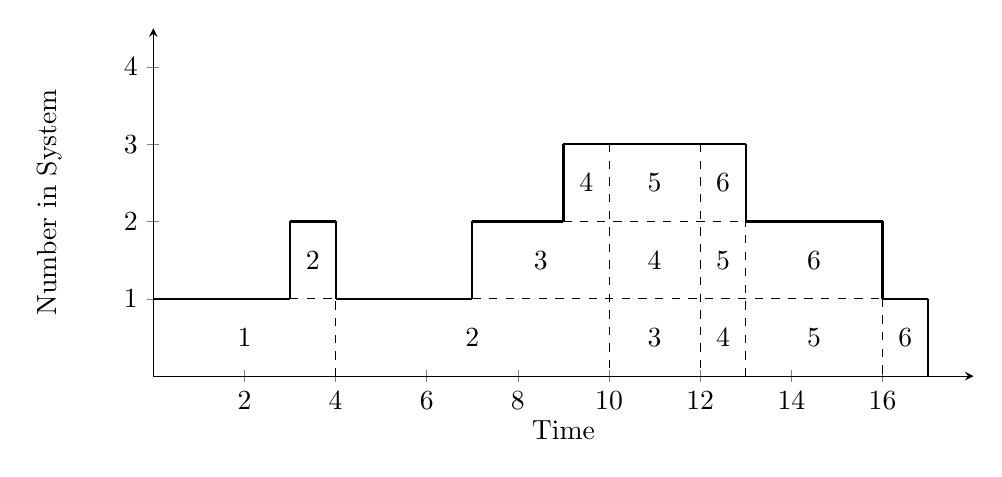
\begin{tikzpicture}[scale=1.0]
    \begin{axis}[clip=false,
      width=12cm, height=6cm,
    axis x line=middle,
    axis y line=middle,
    ymin=0, ymax=4.5,
    ytick={0,1,2,3,4},
    yticklabels={0,1,2,3,4},
    xmin=0, xmax=18,
    xtick={2,4,6,8,10,12,14,16},
    xticklabels={2,4,6,8,10,12,14,16},
    x label style={at={(axis description cs:0.5,-0.1)},anchor=north},
    y label style={at={(axis description cs:-0.1,.5)},rotate=90,anchor=south},
    xlabel=Time,
    ylabel=Number in System,
    ]
    \addplot[mark=none, style=thick] coordinates { (0, 1) (3, 1) };
    \addplot[mark=none, style=thick] coordinates { (3, 1) (3, 2) };
    \addplot[mark=none, style=thick] coordinates { (3, 2) (4, 2) };
    \addplot[mark=none, style=thick] coordinates { (4, 1) (4, 2) };
    \addplot[mark=none, style=thick] coordinates { (4, 1) (7, 1) };
    \addplot[mark=none, style=thick] coordinates { (7, 1) (7, 2) };
    \addplot[mark=none, style=thick] coordinates { (7, 2) (9, 2) };
    \addplot[mark=none, style=thick] coordinates { (9, 2) (9, 3) };
    \addplot[mark=none, style=thick] coordinates { (9, 3) (13,3) };
    \addplot[mark=none, style=thick] coordinates { (13, 3) (13,2) };
    \addplot[mark=none, style=thick] coordinates { (13,2) (16,2) };
    \addplot[mark=none, style=thick] coordinates { (16,2) (16,1) };
    \addplot[mark=none, style=thick] coordinates { (16,1) (17,1) };
    \addplot[mark=none, style=thick] coordinates { (17,1) (17,0) };

    \addplot[mark=none,dashed] coordinates { (3,1) (4,1) };
    \addplot[mark=none,dashed] coordinates { (7,1) (16,1) };
    \addplot[mark=none,dashed] coordinates { (9,2) (13,2) };
    \addplot[mark=none,dashed] coordinates { (10,3) (10,0) };
    \addplot[mark=none,dashed] coordinates { (12,3) (12,0) };
    \addplot[mark=none,dashed] coordinates { (16,1) (16,0) };
    \addplot[mark=none,dashed] coordinates { (4,0) (4,1) };
    \addplot[mark=none,dashed] coordinates { (13,0) (13,2) };

    \node at (2,.5) {1};
    \node at (3.5,1.5) {2};
    \node at (8.5,1.5) {3};
    \node at (9.5,2.5) {4};
    \node at (7,.5) {2};
    \node at (11,.5) {3};
    \node at (11,1.5) {4};
    \node at (11,2.5) {5};
    \node at (12.5,.5) {4};
    \node at (12.5,1.5) {5};
    \node at (12.5,2.5) {6};
    \node at (16.5,.5) {6};
    \node at (14.5,.5) {5};
    \node at (14.5,1.5) {6};

  \end{axis}
\end{tikzpicture}
\end{center}

First note that the problem description does \emph{not} tell us that
the times between arrivals and/or the service times are exponentially
distributed. So it is not an $M/M/1$ system.
The total delay of all six customers is $0+1+3+3+3+4=14$. The average
waiting time in the queue is the total delay divided by the number
of customers.
\[ W_q = \frac{14}{6} = 2.3333~\text{min} \]
To compute the average number in the queue, weight the time in queue
by the number of customers. In other words, compute the area under the
curve but above one, and then divide by the total time.
\[ L_q = \frac{14}{17} \]
\end{solution}

% re-written by hannah.
\item \emph{Justification for a capital expense.} An amusement park is
  known for having rides with short waiting times. A new ride has
  opened, and customers arrive to the ride according to a Poisson
  process with a mean of 20 arrivals per hour. Only one customer is
  allowed on the ride at a time, and customers can stay on the ride as
  long they wish. The length of time that each customer spends on the
  ride is exponentially distributed with a mean of 2.5
  minutes. Management is willing to add an additional cart to the ride
  if, under the current system, 1) the average number of waiting
  customers is greater than four, and 2) the percentage of time that
  the ride is idle exceeds 10\%.  Can an additional cart be justified?

\begin{solution}
  \bs The amusement ride can be modeled as an M/M/1 queuing
  system. Customers arrive at the rate
\[ \lambda = 20~\text{customers per hour,} \]
and the service rate is 
\[ \mu = 24~\text{customers per hour.} \]
To see whether the first condition is satisfied, we compute
\[ L_q = \frac{\lambda^2}{\mu(\mu-\lambda)} = \frac{20^2}{24(24-20)} =
  25/6 > 3~\text{customers} \] 
and so the first condition is satisfied. To
see if the second condition is satisfied, we compute
\[ p_0 = 1 - \frac{\lambda}{\mu} = 0.167 \]
and so the second condition is also satisfied.
\end{solution}

% re-written be hannah
\item \emph{Comparing system configurations.}  Patients arrive to an
  emergency room according to a Poisson process at the rate of 10
  patients per hour. Before a patient can see a doctor, they must have
  their medical history reviewed and their vitals measured. Currently,
  the hospital has one nurse who performs both of these tasks for each
  patient. The time that each patient spends with the nurse is
  exponentially distributed with a mean of five minutes. An Industrial
  Engineer at the hospital is considering two options for improving
  service.
\begin{compactenum}
\item Hire a medical scribe to review each patient's medical history
  while the nurse takes vitals. The service rate would increase to 20
  patients per hour with this improved single-server operation
(service times are still exponentially distributed.) \label{ex:scribe}
\item Hire a second nurse who also reviews medical history and takes
  vitals for each patient. The two nurses would each have a service
  rate of 12 patients per hour (each with exponential service times)
  with this two-server operation.
\end{compactenum}
Consider the relative cost of each option and evaluate the
improvements that would result. Then, determine which option the
engineer should recommend.

\begin{solution}
  \bs We will look at the average number of patients in the queue
  $L_Q$ and the average time in queue $W_Q$ as metrics to judge
  improvement in system performance. Before any improvements are made,
\[ L_q = \frac{\lambda^2}{\mu(\mu-\lambda)} = \frac{10^2}{12(12-10)} = 25/6 = 4.167~\text{patients} \]
and
\[W_q = \frac{L_q}{\lambda} = \frac{25/6}{10} = 5/12~\text{hours} = 25~\text{minutes} \]
If they hire a scribe to assist the nurse
\[ L_q = \frac{\lambda^2}{\mu(\mu-\lambda)} = \frac{10^2}{20(20-10)} = 0.5~\text{patients} \]
and
\[W_q = \frac{L_q}{\lambda} = \frac{0.5}{10} = 0.05~\text{hours} =
  3~\text{minutes} \] 
and if they add an additional nurse we need to
use the formulas for a two-server operation. First,
\[ P_0 = \frac{1}{\sum_{n=0}^{k-1}\frac{\left(\lambda/\mu\right)^n}{n!} + \frac{\left(\lambda/\mu\right)^k}{k!}\left(\frac{k\mu}{k\mu-\lambda}\right)} \]
where $k=2$ servers. Then
\[ L_q = \frac{\left(\lambda/\mu\right)^k\lambda\mu}{(k-1)!(k\mu-\lambda)^2}P_0 \]
and
\[W_q = \frac{L_q}{\lambda} \] 
Plugging values, I got $P_0=0.4118$,
$L_q=0.1751$ patients, and $W_q=0.0175$ hours or $1.05$ minutes.
Considering the relative improvement and the cost of adding a second
nurse, I would recommend option~\ref{ex:scribe}. That is, to hire a scribe to help
the nurse. The average number in queue and the average time in queue
appear to be acceptable for an emergency room setting.
\end{solution}

% the context of this problem needs to be re-written. perhaps describe a
% situation of a store with two clerks, each with exponential service times
% (so total service time is Gamma/Erlang). Social distancing measures mean
% that only one customer at a time is allowed in the store.
\item \emph{An $M$/$G$/$1$ queue.}  A coffee shop has recently opened
  for takeout after being closed due to COVID-19. In order to follow
  public health guidelines, only one customer is allowed in the shop
  at a time. If a customer is being served, any customer
  that arrives must wait in a line outside of the coffee
  shop. Customers arrive at a rate of 12 customers per hour, and
  inter-arrival times are exponentially distributed. The shop has two
  baristas: one barista takes orders and the other prepares the
  beverages. The service time for each barista to complete their task
  is independently and exponentially distributed with a mean of two
  minutes. Determine the average number of customers waiting in line
  to be served, $L_Q$. A couple of helpful items:
\begin{compactenum}[i)]
\item The variance of the sum of independent
random variables is the sum of the variances,
\item the sum of IID
exponential random variables is distributed Gamma, 
\item the variance
of an exponential distribution is the mean squared, and
\item for an $M$/$G$/1 queue, 
\[ L_Q = \frac{\rho^2(1 + \sigma^2\mu^2)}{2(1-\rho)} \]
where $\rho$ is the server utilization, $\mu$ is the service rate, and $\sigma^2$ is
the variance of the service time distribution.
\end{compactenum}

\begin{solution}
\bs The first thing to note is that the service time is the sum of two IID exponential
random variables, and so we know that it has a Gamma distribution.
Letting $X$ represent the service time,
\[ \text{Var}(X) = 2^2 + 2^2 = 8.\]
The expected total service time for both baristas is 4 minutes, so
$\mu = 1/4$ customers per minute. 
Now, in units of customers per minute, the arrival rate is $\lambda = 1/5$.
\begin{align*}
      L_Q &= \frac{\frac{16}{25}\left(1 + 8\left(\frac{1}{16}\right)\right)}{2\left(\frac{1}{5}\right)} \\
      &= 2.4 ~\text{customers}
\end{align*}
\end{solution}


\subsubsection*{Stochastic Dynamic Programming}

\subsubsection*{Probabilistic Inventory Models}

% written by Emily
% Probabilistic Inventory Model

\item \emph{Stocking a seasonal item.} Summer is approaching and a
  store is determining how many folding lawn chairs they should
  purchase from a supplier.  Each chair costs \$15\ for the store to
  purchase and can be sold for \$27.50.\ The store stocks lawn chairs
  only during the summer; any chairs left at the end of the summer are
  sold at a clearance price of \$10.50.\ Based on historical data, the
  seasonal summer demand for lawn chairs follows a normal distribution with
  $\mu = 205$ and $\sigma = 25$.

\begin{enumerate}
\item What is your recommended order quantity for the store?
\item What is the probability that the store will sell all the folding
  lawn chairs it orders before summer is over? \label{ex:lawn}
\item How would the economic order quantity change if the clearance
  price for the chairs was only \$8?\ What happens to the store's
  order quantity as the clearance price is reduced? \label{ex:clearance}
\end{enumerate}

\begin{solution}
  \bs Let $D$ be the summer demand for folding lawn chairs. We know
  that $D \sim \mathcal{N}\left(\mu=205,~\sigma=25\right)$. The
  penalty for ordering too few items is $c_u= 12.50$ and the penalty
  for ordering too many items is $c_o= 4.50$. We want to find the
  order quantity $Q^{\ast}$ such that


\[ P\left(D \leq Q^{\ast}\right) < \frac{c_u}{c_u+c_o} = \frac{12.50}{17.00} = 0.735 \]
Standardizing,
\[ P\left(z \leq \frac{Q^{\ast}-205}{25}\right) = 0.735 \]
implies that
\begin{align*}
\frac{Q^{\ast}-205}{25} &= 0.63 \\
Q^{\ast} &= 205 + 0.63(25)\\
Q^{\ast} &= 220.75
\end{align*}

The store should order 221 (or 220) folding lawn chairs. 
If we are using R, we can obtain the answer without standardizing
by simply passing the mean and standard deviation to \texttt{qnorm},
\begin{Verbatim}
> qnorm(.735, 205, 25)
[1] 220.7002
\end{Verbatim}

For part~\ref{ex:lawn}, the probability that all chairs will sell is


\begin{align*}
  P\left(D \geq 221 \right) &= 1 - P\left(D \leq 221 \right)\\
                            &= 1 - P\left( z \leq \frac{221-205}{25} \right) \\
                            &= 1 - P\left( z \leq .64 \right)\\
                            &= 1 - .74 \\
                            &= 0.26
\end{align*}


Regarding part~\ref{ex:clearance}, if the clearance price decreases to
\$8\, then the cost of being under-stocked will still be $c_u=12.50$,
but the cost of being over will increase to $c_o=7.00$. The order
quantity $Q^{\ast}$ will change such that

\begin{align*}
  P\left(D \leq Q^{\ast}\right) = \frac{12.50}{19.50} &= .641 \\
  P\left(z \leq \frac{Q^{\ast}-205}{25}\right) &= .641
\end{align*}
which implies that
\begin{align*}
  \frac{Q^{\ast}- 205}{25} &= .36\\
  Q^{\ast} &= 205 + 0.36(25) = 214
\end{align*}

With a clearance price of \$8, the new order quantity will be 214
chairs.  The economic order quantity will continue to decrease as the
clearance price decreases because the cost of being over will continue
to increase.
\end{solution}

% written by Emily
% Uniform distribution
\item \emph{Programs for sale.}  A college hockey team has game
  programs for sale at every home game they play. The demand $D$ for
  these programs is a random variable that follows a Uniform
  distribution with a minimum of \num{1200} programs and a maximum of
  \num{2000} programs.
  \[ D \sim \text{Uniform}(1200,\,2000) \] Each program costs \$1\ to
  produce and sells for \$3.\ The programs contain information
  specific to the game, so any unsold programs are thrown away after
  the game. How many game programs should the college print per game
  to maximize their revenue? You should use the CDF of the Uniform
  distribution to answer this question.
  
\begin{solution}
\bs 
The CDF of Uniform distribution is
\[ P(X \leq x) = F(x) = \int_{y=a}^x f(y)\,dy = \int_{y=a}^x
  \frac{1}{b-a}\,dy = \frac{x-a}{b-a} \] for $a \leq x \leq b$.  The
cost per copy of being over/under is $c_o = \$1$ and $c_u = \$2$,
respectively.  Let $Q^{\ast}$ be the optimal number of copies to
produce.  Using the critical ratio, we want
\[ P\left(D \leq Q^{\ast}\right) = \frac{c_u}{c_u+c_o} = 
\frac{2}{3} \approx 0.667 \]
Using the definition of the CDF for the Uniform distribution,
\begin{align*}
  \frac{Q^{\ast} - 1200}{2000-1200} &= 0.667 \\
    Q^{\ast} &= 0.667\times 800 + 1200\\
    Q^{\ast} &= 1734
\end{align*}
The college should print 1734 copies.
\end{solution}

% written by Emily
\item \emph{The risk of being out-of-stock.}
The daily demand for milk cartons in a school cafeteria
follows a Normal distribution with mean 600 and standard
deviation 20. It costs \$.01 per day to hold one item in
inventory. The fixed cost to make a replenishment order is
\$50, and the lead time to receive an order is 2 days.

\begin{enumerate}
\item Currently, the inventory policy for milk cartons is 
to order \num{3000} cartons whenever the inventory drops 
to \num{1225} units. Determine the probability of a 
stock-out under this policy. \label{ex:pol}

\item Running out of milk generates lots of complaints to the
PTA. Recommend an inventory policy for the school when
the probability of a stock-out cannot exceed .01.
Your policy should include an economic order quantity and 
a re-order point.
\label{ex:so-policy}

\item Compare the cost of the policy in part~\ref{ex:pol} with 
the cost of the policy in part~\ref{ex:so-policy}. \label{ex:comp-pol}
\end{enumerate}

\begin{solution}
\bs The distribution of demand during lead time $X_m$ is
\[ X_m \sim \text{Normal}(\mu_m=1200,\sigma_m=\sqrt{800}) \]
The probability of a stock-out is
\begin{align*}
  P(X_m \geq 1225) &= P\left(z \geq \frac{1225-\mu_m}{\sigma_m}\right) \\
                  &= 1 - P\left(z < \frac{1225-1200}{\sqrt{800}}\right) \\
                  &= 1 - P\left(z < 0.8839\right) \\
                  &= 1 - .8106 \\
                  &\approx .19
\end{align*}

With the requirement that the probability of a stock-out not exceed
0.01, the optimal order quantity is
\[
  Q^{\ast} = \sqrt{\frac{2C_oD}{C_h}} = 
  \sqrt{\frac{2\times 50\times 600}{.01}} \approx 2450
\]
Without a buffer stock the optimal policy is to order 
\num{2400} milk cartons every $T_0=Q^{\ast}/D \approx 4$ days. 
To compute the buffer stock, we want
\[
  P(X_m \geq B + 1200) \leq 0.01
\]
or equivalently, we want $B \geq \sigma_m \times 
2.33 \approx 66$.
The best policy is to order \num{2400} milk cartons 
whenever the inventory drops to $\num{1200}+66=\num{1266}$ units.

On average, the total daily cost of the current inventory policy (not
considering the frustration costs of a stock-out) consists of the
holding cost and the ordering cost. The holding cost has two terms:
one for the normal inventory and one for the buffer stock
\begin{align*}
 & \left(\frac{Q}{2}\right)\left(C_h\right)  + \left(25\right)\left(C_h)\right)\\
= & \left(\frac{3000}{2}\right)\left(0.01\right) + (25)(0.01) \\
= & \$15 + \$0.25 \\
= & \$15.25 ~\text{per day.}
\end{align*}
The ordering cost of the current policy is
\[ \left(\frac{600}{3000}\right) \left(50\right) = \$10~\text{per
    day.} \] Remember that demand is random and so these costs are
``on average''.  The only difference in cost for the new inventory
policy in part~\ref{ex:so-policy} is the increased holding cost for
the larger buffer stock. This amounts to an increase of
\[ (66 - 25) (0.01) = \$0.41~\text{per day.} \]
Assuming the milk does not expire before it is used, the benefit
of fewer stock-outs seems to be worth the increase in cost.
\end{solution}

\end{enumerate}
